\documentclass{article}
% Some basic packagesLLuu
\usepackage[utf8]{inputenc}
\usepackage{spverbatim}
\usepackage[margin=1.2in]{geometry}
\usepackage{textcomp}
\usepackage{url}
\usepackage{graphicx}
\usepackage{float}
\usepackage{algorithm2e}
% \usepackage{algorithm}
\usepackage{enumitem}
\usepackage{standalone}
\usepackage{tcolorbox}
\usepackage{wrapfig}
% \usepackage{svg}
% \usepackage{svg-inkscape} 

\graphicspath{{./figures}}


%color settings
\usepackage{xcolor}
% \definecolor{gruvbgdark}{HTML}{1d2021}
% \definecolor{gruvtextdark}{HTML}{ebdbb2}
% \definecolor{gruvbglight}{HTML}{f9f5d7}
% \definecolor{gruvtextlight}{HTML}{3c3836}
% \definecolor{NavyBlue}{HTML}{266bbd}
% \definecolor{RawSienna}{HTML}{94330e}
% \definecolor{ForestGreen}{HTML}{149b52}
% \pagecolor{gruvbgdark}
% \color{gruvtextdark}

\definecolor{GBBlue}{HTML}{458588}
\definecolor{GBGreen}{HTML}{98971A}
\definecolor{GBRed}{HTML}{CC241D}
\definecolor{GBYellow}{HTML}{D79921}
\definecolor{GBPurple}{HTML}{B16286}
\definecolor{GBAqua}{HTML}{689D6A}
\definecolor{GBOrange}{HTML}{D65D0E}
\definecolor{GBGray}{HTML}{A89984}
\definecolor{GBDarkGray}{HTML}{3C3836}
\definecolor{GBLightGray}{HTML}{EBDBB2}
\definecolor{GBBackground}{HTML}{282828}
\definecolor{GBForeground}{HTML}{FBF1C7}
\pagecolor{GBBackground}
\color{GBForeground}
% Hide page number when page is empty
\usepackage{emptypage}
\usepackage{subcaption}
\usepackage{multicol}

% Math stuff
\usepackage{amsmath, amsfonts, mathtools, amsthm, amssymb}
% Fancy script capitals
\usepackage{mathrsfs}
\usepackage{cancel}

% Bold math
\usepackage{bm}

%Algorithm setup
\RestyleAlgo{algoruled}
% Some shortcuts
\newcommand\N{\ensuremath{\mathbb{N}}}
\newcommand\R{\ensuremath{\mathbb{R}}}
\newcommand\Z{\ensuremath{\mathbb{Z}}}
\renewcommand\O{\ensuremath{\emptyset}}
\newcommand\Q{\ensuremath{\mathbb{Q}}}
\newcommand\C{\ensuremath{\mathbb{C}}}
\newcommand\B{\ensuremath{\mathbb{B}}}

%Make implies and impliedby shorter
\let\implies\Rightarrow
\let\impliedby\Leftarrow
\let\iff\Leftrightarrow


% Add \contra symbol to denote contradiction
% \usepackage{stmaryrd} % for \lightning
% \newcommand\contra{\scalebox{1.5}{$\lightning$}}

\let\phi\varphi

% Command for short corrections
% Usage: 1+1=\correct{3}{2}

\definecolor{correct}{HTML}{009900}
\newcommand\correct[2]{\ensuremath{\:}{\color{red}{#1}}\ensuremath{\to }{\color{correct}{#2}}\ensuremath{\:}}
\newcommand\green[1]{{\color{correct}{#1}}}

% horizontal rule
% \newcommand\hr{
%     \noindent\rule[0.5ex]{\linewidth}{0.5pt}
% }

% hide parts
\newcommand\hide[1]{}

% Environments
\makeatother

% For box around Definition, Theorem, \ldots
% theorems
\usepackage{thmtools}
\usepackage[framemethod=TikZ]{mdframed}
\mdfsetup{skipabove=1em,skipbelow=1em, innertopmargin=5pt, innerbottommargin=6pt}

\theoremstyle{definition}

\makeatletter

\declaretheoremstyle[headfont=\bfseries, bodyfont=\normalfont, numbered=no]{idea}

\declaretheoremstyle[
	headfont=\bfseries\color{ForestGreen!70!black}, bodyfont=\normalfont,
    postheadspace=\newline,
	mdframed={
			linewidth=2pt,
			rightline=false, topline=false, bottomline=false,
			linecolor=ForestGreen, backgroundcolor=ForestGreen!5,
		},
    numberwithin=section
]{thmgreenbox}

\declaretheoremstyle[
	headfont=\bfseries\color{NavyBlue!70!black}, bodyfont=\normalfont,
    postheadspace=\newline,
	mdframed={
			linewidth=2pt,
			rightline=false, topline=false, bottomline=false,
			linecolor=NavyBlue, backgroundcolor=NavyBlue!5,
		},
    numberwithin=section
]{thmbluebox}
\declaretheoremstyle[
	headfont=\bfseries\color{NavyBlue!70!black}, bodyfont=\normalfont,
	mdframed={
			linewidth=2pt,
			rightline=false, topline=false, bottomline=false,
			linecolor=NavyBlue, backgroundcolor=NavyBlue!5,
		},
    numberwithin=section
]{thmclaimbox}

\declaretheoremstyle[
	headfont=\bfseries\color{NavyBlue!70!black}, bodyfont=\normalfont,
	mdframed={
			linewidth=2pt,
			rightline=false, topline=false, bottomline=false,
			linecolor=NavyBlue
		},
    numberwithin=section
]{thmblueline}

\declaretheoremstyle[
	headfont=\bfseries\color{RawSienna!70!black}, bodyfont=\normalfont,
    postheadspace=\newline,
	mdframed={
			linewidth=2pt,
			rightline=false, topline=false, bottomline=false,
			linecolor=RawSienna, backgroundcolor=RawSienna!5,
		},
    numberwithin=section
]{thmredbox}

\declaretheoremstyle[
	headfont=\bfseries\color{RawSienna!70!black}, bodyfont=\normalfont,
    postheadspace=\newline,
	mdframed={
			linewidth=2pt,
			rightline=false, topline=false, bottomline=false,
			linecolor=RawSienna, backgroundcolor=RawSienna!5,
		},
	qed=\qedsymbol,
    numberwithin=section
]{thmproofbox}

\declaretheoremstyle[
	headfont=\bfseries\color{NavyBlue!70!black}, bodyfont=\normalfont,
	numbered=no,
	mdframed={
			linewidth=2pt,
			rightline=false, topline=false, bottomline=false,
			linecolor=NavyBlue, backgroundcolor=NavyBlue!1,
		},
]{thmexplanationbox}

\declaretheorem[style=thmgreenbox, name=Definition]{definition}
\declaretheorem[style=thmbluebox, numbered=no, name=Problem Statement]{stmt}
\declaretheorem[style=thmbluebox, numbered=no, name=Answer]{ans}
\declaretheorem[sibling=definition, style=thmredbox, name=Corollary]{corollary}
\declaretheorem[style=thmbluebox, numbered=no, name=Idea]{idea}
\declaretheorem[style=thmbluebox,  name=Proposition]{prop}
\declaretheorem[style=thmredbox, name=Theorem]{theorem}
\declaretheorem[style=thmproofbox, name=Proof]{prf}
\declaretheorem[style=thmredbox, name=Lemma]{lemma}
\declaretheorem[style=thmclaimbox, numbered=no, name=Claim]{claim}
\declaretheorem[numbered=no, style=thmexplanationbox, name=Proof]{explanation}
\declaretheorem[numbered=no, style=thmproofbox, name=Proof]{replacementproof}
\declaretheorem[style=thmgreenbox,  numbered=no, name=Task]{ex}
\declaretheorem[style=thmbluebox,  numbered=no, name=Example]{eg}
\declaretheorem[style=thmblueline, numbered=no, name=Remark]{remark}
\declaretheorem[style=thmblueline, numbered=no, name=Note]{note}

\renewenvironment{proof}[1][\proofname]{\begin{replacementproof}}{\end{replacementproof}}
\AtEndEnvironment{eg}{\null\hfill$\diamond$}%

\newtheorem*{uovt}{UOVT}
\newtheorem*{notation}{Notation}
\newtheorem*{previouslyseen}{As previously seen}
\newtheorem*{problem}{Problem}
\newtheorem*{observe}{Observe}
\newtheorem*{property}{Property}
\newtheorem*{intuition}{Intuition}

\newcommand{\oefening}[1]{%
	\def\@oefening{#1}%
	\subsection*{Oefening #1}
}

\newcommand{\suboefening}[1]{%
	\subsubsection*{Oefening \@oefening.#1}
}


% \lecture starts a new lecture (les in dutch)
%
% Usage:
% \lecture{1}{di 12 feb 2019 16:00}{Inleiding}
%
% This adds a section heading with the number / title of the lecture and a
% margin paragraph with the date.

% I use \dateparts here to hide the year (2019). This way, I can easily parse
% the date of each lecture unambiguously while still having a human-friendly
% short format printed to the pdf.

% \usepackage{xifthen}
% \def\testdateparts#1{\dateparts#1\relax}
% \def\dateparts#1 #2 #3 #4 #5\relax{
% 	\marginpar{\small\textsf{\mbox{#1 #2 #3 #5}}}
% }

% \def\@lecture{}%
% \newcommand{\lecture}[3]{
% 	\ifthenelse{\isempty{#3}}{%
% 		\def\@lecture{Lecture #1}%
% 	}{%
% 		\def\@lecture{Lecture #1: #3}%
% 	}%
% 	\subsection*{\@lecture}
% 	% \marginpar{\small\textsf{\mbox{#2}}}
% }

\usepackage{listings}

\definecolor{dkgreen}{rgb}{0,0.6,0}
\definecolor{gray}{rgb}{0.5,0.5,0.5}
\definecolor{mauve}{rgb}{0.58,0,0.82}

\lstset{frame=single,
  language=c,
  aboveskip=3mm,
  belowskip=3mm,
  showstringspaces=false,
  columns=flexible,
  basicstyle={\small\ttfamily},
  numbers=none,
  numberstyle=\tiny\color{GBForeground},
  keywordstyle=\color{GBRed},
  commentstyle=\color{GBGreen},
  stringstyle=\color{GBAqua},
  breaklines=true,
  breakatwhitespace=true,
  tabsize=2
}



% These are the fancy headers
\usepackage{fancyhdr}
\pagestyle{fancy}

% LE: left even
% RO: right odd
% CE, CO: center even, center odd
% My name for when I print my lecture notes to use for an open book exam.
\fancyhead[LE,RO]{Kristian Sørdal}

\fancyhead[RO,LE]{INF236 - Parallel Programmering} % Right odd,  Left even
% \fancyhead[RE,LO]{\leftmark}          % Right even, Left odd
\fancyhead[RE,LO]{Kristian Sørdal}          % Right even, Left odd

% \fancyfoot[RO,LE]{\thepage}  % Right odd,  Left even
% \fancyfoot[RE,LO]{Kristian Sørdal}          % Right even, Left odd
% \fancyfoot[C]{\leftmark}     % Center

\makeatother

% Todonotes and inline notes in fancy boxes
\usepackage{todonotes}
\usepackage{tcolorbox}

% Make boxes breakable
\tcbuselibrary{breakable}

% Figure support as explained in my blog post.
\usepackage{import}
\usepackage{xifthen}
\usepackage{pdfpages}
\usepackage{transparent}
\newcommand{\incfig}[2][1]{%
	% \begin{center}
	\def\svgwidth{#1\columnwidth}
	\import{./figures/}{#2.pdf_tex}
	% \end{center}
}
% Fix some stuff
% %http://tex.stackexchange.com/questions/76273/multiple-pdfs-with-page-group-included-in-a-single-page-warning
\pdfsuppresswarningpagegroup=1
\author{Kristian Sørdal}


\title{Assignment 3 - Sparse Matrix Vector Multiplication}
\author{Kristian Sørdal}
\begin{document}
\maketitle
\newpage
\tableofcontents
\newpage
    % \section{Benchmark}
    \section{Sparse Matrix Vector Multiplication (SpMV)}
    Sparse Matrix Vector Multiplication (SpMV) is a common operation used in scientific computing. It lends itself very well to parallelization, both in shared and distributed memory systems. The matrices used in SpMV are usually very big, typically on the order of at least \( 10^{8} \) rows, with at least \( 10^{9} \) non-zeros.
    \medskip

    Although there are many definitions as to what a sparse matrix is, they all generally describe matrices where its worth treating non-zeros differently to zeros. For the matrices used in this project, we will be working with matrices with \( \mathcal{O}\left(n\right) \) non-zeros, i.e. \( \mathcal{O}\left(1\right) \) non-zeros per row. Below is an example of a sparse matrix.

    \begin{figure}[H]
        \begin{center}
\begin{align*}
\begin{array}{cc}
    \begin{bmatrix}
         1&5&0&0&4&0&0&1  \\
         0&7&0&9&0&12&0&0  \\
         0&8&7&0&0&0&0&0  \\
         0&0&0&0&0&3&3&17  \\
         0&0&0&2&2&0&1&0  \\
         0&0&0&0&0&6&0&0  \\
    \end{bmatrix}
    &
    \begin{bmatrix}
         1&5&&&4&&&1  \\
         &7&&9&&12&&  \\
         &8&7&&&&&  \\
         &&&&&3&3&17  \\
         &&&2&2&&1&  \\
         &&&&&6&&  \\
    \end{bmatrix} \\
    \text{A} & \text{A}
\end{array}
\end{align*}
        \end{center}
        \caption{(Left) Dense representation of A , (Right) Sparse representation of A} %Matrix remains the same, left is represented as a dense matrix, right as a sparse matrix.}
    \end{figure}

    \subsection{Representing a Sparse Matrix effectively}
    There are many different ways to represent a sparse matrix. The key takeway from all of them is that they don't store the zeros. For this project, the Compressed Sparse Row (CSR) format  has been utilized. Storing a matrix using this format, we need 3 vectors. The \texttt{row\_ptr} vector has size \( n + 1 \), where the \( i \)th entry represents the starting index in the \texttt{col\_idx} vector of the \texttt{i}th row. The \texttt{col\_idx} vector has size \( nnz \), where \( nnz \) is the number of non-zeros in the matrix. It represents the presence of a non-zero values in the matrix. If \texttt{col\_idx[4]} = 5, then the matrix has a non-zero value at index \( [4,5] \). Finally, the \texttt{vals} vector also has size \( nnz \), and it stores the numerical value of the non-zeros. Below is an example of a sparse matrix, and the CSR representation of the same matrix.

    \begin{figure}[H]
        \centering
            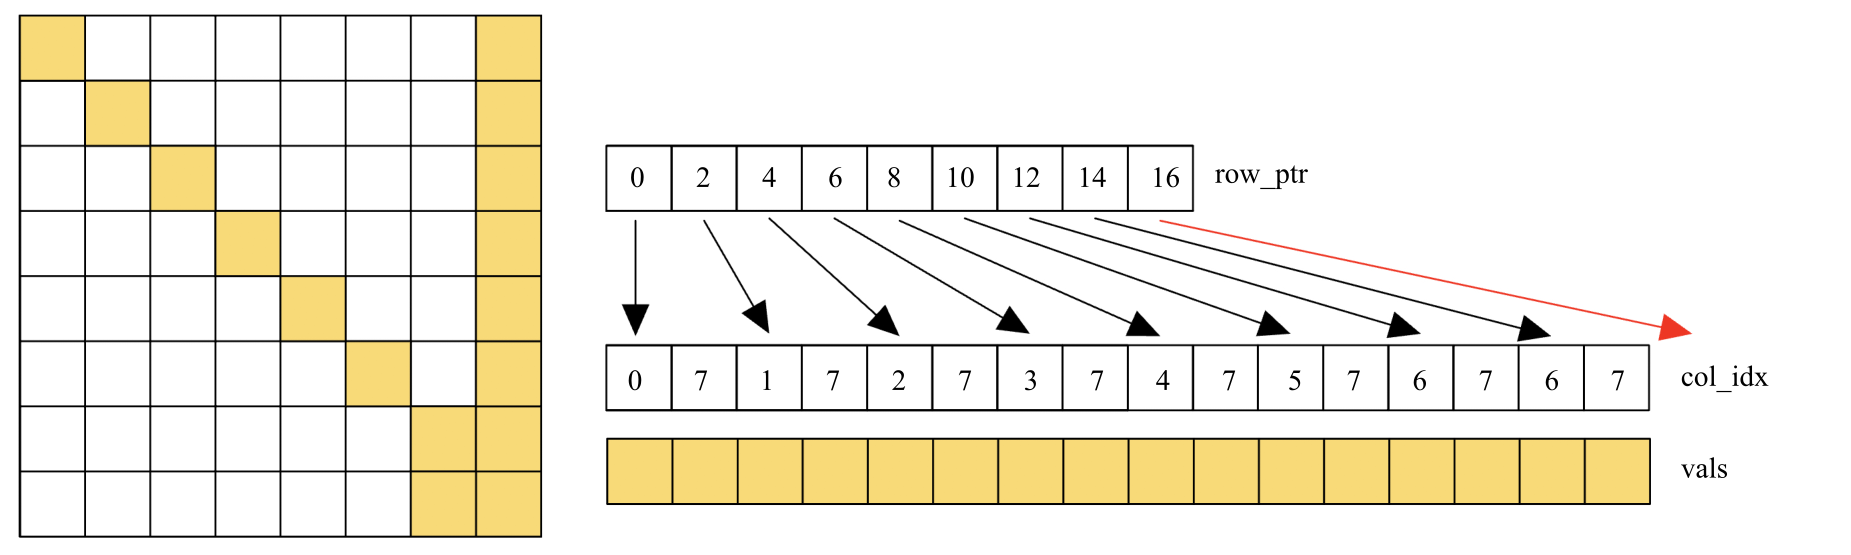
\includegraphics[width=\textwidth]{matrixcsr}
        \caption{Compressed Sparse Row Format}
    \end{figure}

    \newpage
    \subsection{SpMV Kernel}

    The kernel used for computing the result of an iteration of SpMV on a CSR matrix is outlined in the algorithm below. This is what will be parallelized in order to (hopefully) achieve better performance.
    \medskip

    \begin{algorithm}[H]
        \caption{SpMV Kernel}
        \SetAlgoVlined
        \SetKwInOut{Input}{Input}
        \SetKwInOut{Output}{Output}
        \Input{Row pointer: \textit{rowPtr}, Column indices: \textit{colIdx}, Values: \textit{vals}, Input vector \( x \), Result vector \( y \) }
        \Output{Output Vector \( y \)\newline}

        \For{\(row \leftarrow 0 \) \KwTo \( n \)}{
            \For{\(idx \leftarrow rowPtr[row] \) \KwTo \( rowPtr[row + 1] \)}{
                \( y[row] \leftarrow y[row] + vals[idx] \times x[colIdx[idx]] \)
            }
        }
    \end{algorithm}

    \section{STREAM Benchmark}
    When performing SpMV with the CSR format, we have to be aware that the performance of our program will likely not scale with the number of threads we throw at the program, but rather the memory bandwidth of the system we are running on. Memory bandwidth is the rate at which data can be read or stored in memory. The reason for this becomes evident when we look at the kernel.
    \medskip

    When we execute the kernel, we are repeatedly accessing memory, and do very few operations (just 2 floating point operations) per memory access. In addition to this, we are accessing the input vector \texttt{x} in a manner that leads to a large amount of cache misses. This is because it is indexed by the value stored in \texttt{col\_idx}. Although this vector is sorted in increasing order when looking at a single row, the indices stored in this vector can, and usually will have a large difference in their numerical value. When we access any value at a given index in the \texttt{x} vector, the processor will prefetch successive elements in this vector and load them into the cache, allowing for very fast access. But since the numerical difference between the indices can be large, most likely the next element we need will not be prefetched, thus requiring the processor to read the value from memory, instead of reading from the cache. It is for this reason that SpMV is limited by the memory bandwidth of the system.
    \medskip

    The STREAM is an industry standard benchmark that is used for measuring sustained memory bandwidth of the CPU in a shared memory system. The benchmark computes four different kernels named \texttt{Copy}, \texttt{Scale}, \texttt{Sum} and \texttt{Triad}. The kernels are defined as the following:

    \begin{itemize}
        \item Copy: \( y[i] = x[i] \)
        \item Scale: \( y[i] = \alpha \times x[i] \)
        \item Sum: \( y[i] = x[i] + y[i] \)
        \item Triad: \( y[i] = x[i] + \alpha \times z[i] \)
    \end{itemize}
        
    We are interested in the results from the \texttt{Triad} kernel, as this is the only kernel which uses 2 FLOPS per iteration, which is the same as we do in SpMV.
    \medskip

    By running the STREAM benchmark on Brake and plotting the results, we can see the sustained memory bandwidth achieved for each thread. This will be important for comparing the results of the different implementations of parallel SpMV later on. Below we can see the results of the benchmark.

    \begin{figure}[H]
        \begin{center}
            \includegraphics[width=0.95\textwidth]{stream.png}
        \end{center}
        \caption{Results of STREAM Benchmark - Triad kernel.}
    \end{figure}
    \begin{figure}[H]
        \begin{center}
            \includegraphics[width=0.95\textwidth]{streamgf.png}
        \end{center}
        \caption{Results of STREAM Benchmark - Triad kernel, GFLOPS}
    \end{figure}

    As we can see, we are able to achieve at most \( \approx 33 \) GB/s in sustained memory bandwidth, and a peak of \( \approx 2.5 \) GFLOPS, so we should not expect that the SpMV results will exceed this number.


    \section{Parallelizing SpMV}

    For this project, 3 different strategies were implemented for parallelizing SpMV. The following sections will discuss their implementation details. 

    \subsection{Method 1}

    This method is the simplest of all methods, as it simply parallelizes the outmost for-loop of the kernel, using OpenMP's \texttt{\#pragma omp parallel for} directive. From testing different scheduling methods, it was found that \texttt{dynamic} scheduling with a block size of 1024 was the best choice. The kernel now looks like the following:
    \medskip


    \begin{algorithm}[H]
        \caption{SpMV Kernel}
        \SetAlgoVlined
        \SetKwInOut{Input}{Input}
        \SetKwInOut{Output}{Output}
        \Input{Row pointer: \textit{rowPtr}, Column indices: \textit{colIdx}, Values: \textit{vals}, Input vector \( x \), Result vector \( y \) }
        \Output{Output Vector \( y \)\newline}

        \ForPar{\(row \leftarrow 0 \) \KwTo \( n \)}{
            \For{\(idx \leftarrow rowPtr[row] \) \KwTo \( rowPtr[row + 1] \)}{
                \( y[row] \leftarrow y[row] + vals[idx] \times x[colIdx[idx]] \)
            }
        }
    \end{algorithm}

    \subsection{Method 2}
    The next method is slightly more involved, as it makes use of manually assigning rows to each thread, in an attempt at achieving a better load balance for each thread, trying to ensure that no thread does significantly more work than any of the other threads.
    \medskip

    The load balancing strategy used in this method involves computing the ideal number of non-zeros each thread should work on, by dividing the total number of non-zeros by the number of threads. Then for each thread, we greedily assign rows (without splitting them) until the sum of non-zeros in each row is at or just above the ideal number of non-zeros. The algorithm used for this is implemented in the following manner:
    \medskip

    \begin{algorithm}[H]
        \caption{Naive Load Balancing}
        \SetAlgoVlined
        \SetKw{Break}{break}
        \SetKwInOut{Input}{Input}
        \SetKwInOut{Output}{Output}
        \Input{Row pointer: \textit{rowPtr}, Number of non-zeros: \textit{nnz}, Number of threads: \textit{numThreads}, Number of rows: \textit{N},}
        \Output{Start and end indicies for each rank}

        partitionSize \( \leftarrow \) list of size \( p \), assigned tuples \( \left( 0,0 \right) \)\\
        avgNnz \( \leftarrow \frac{nnz}{p} \)\\
        threadIdx \( \leftarrow 0 \)\\
        prevIdx \( \leftarrow 0 \)\\

        \For{i \( \leftarrow 0 \) \KwTo N}{
            \If{threadIdx = numThreads \( -1 \)}{
                partition[threadIdx] \( \leftarrow \) (prevIdx, N)
                \Break
            }
            \If{rowPtr[i+1] - rowPtr[prevIdx] > avgNnz}{
                partition[threadIdx] \( \leftarrow \) (prevIdx,i)
                prevIdx \( \leftarrow \) i
                threadIdx \( \leftarrow \) threadIdx + 1
            }
        }
    \end{algorithm}

    Then, for each thread, we compute the following kernel:
    \medskip

    \begin{algorithm}[H]
        \caption{SpMV Kernel - Load Balanced}
        \SetAlgoVlined
        \SetKwInOut{Input}{Input}
        \SetKwInOut{Output}{Output}
        \Input{Row pointer: \textit{rowPtr}, Column indices: \textit{colIdx}, Values: \textit{vals}, Input vector \( x \), Result vector \( y \), Start index: startIdx, End index: endIdx }
        \Output{Output Vector \( y \)\newline}

        \For{\(row \leftarrow \)startIdx \KwTo endIdx}{
            \For{\(idx \leftarrow rowPtr[row] \) \KwTo \( rowPtr[row + 1] \)}{
                \( y[row] \leftarrow y[row] + vals[idx] \times x[colIdx[idx]] \)
            }
        }
    \end{algorithm}

    \subsection{Method 3}
    The final method implemented makes use of the METIS graph partitioning library, this exposes two methods for paritioning a graph into \( k \) parts. We have the choice of using either multilevel recursive bisection, or \( k \)-way partitioning. After some testing, \( k \)-way partitioning was found to be the most stable, as the multilevel recursive bisection sometimes resulted in segmentation faults. 
    \medskip

    It should be noted that METIS is primarily used to reduce the total communication volume in distributed memory systems, it does this by minimizing the amount of edges that cross from one partition into another. This means that it doesn't necessarily distribute the number of non-zeros each thread has to work on evenly. 
    \medskip

    By using the METIS library, the goal is to hopefully achieve an even better load balance than what the greedy approach described earlier can provide. The algorithm used for load balancing with METIS is outlined below.



    \begin{algorithm}[H]
        \caption{Metis Load Balancing}
        \SetAlgoVlined
        \SetKwComment{Comment}{//}{}
        \SetKw{Break}{break}
        \SetKwInOut{Input}{Input}
        \SetKwInOut{Output}{Output}
        \Input{Number of partitions: \textit{k}, Row pointer: \textit{rowPtr}, Column indices: \textit{colIdx}, Values: \textit{vals},Input vector: inputVec, Number of non-zeros: \textit{nnz}, Number of rows: \textit{N}}
        \Output{Start and end indicies for each rank}

        \phantom{a}\\
        startIdx \( \leftarrow \) 0 initialized list of size \( p + 1 \)\\
        partitionMap \( \leftarrow \) 0 initialized list of size \( N \)\\
        objval \( \leftarrow \) NULL\\
        ncon \( \leftarrow \) 1\\
        ubvec \( \leftarrow \) 1.01\\
        \phantom{a}\\

        \If{k = 1}{
            startIdx[1]=N
            \Return
        }
        rc \( \leftarrow \) METISPartGraphKway(\&N, \&ncon, *rowPtr, *colIdx, nullptr, nullptr, nullptr, \&k, nullptr, \&ubvec, nullptr, \&objval, *partitionMap)\\
        \phantom{a}\\
        newId \( \leftarrow \) 0 initialized list of size \( N \)\\
        oldId \( \leftarrow \) 0 initialized list of size \( N \)\\
        id \( \leftarrow \)0\\

        \Comment { Reenumerate the rows according to the partitionMap} 
        \For{r \( \leftarrow 0 \) \KwTo k}{
            \For{i \( \leftarrow 0 \) \KwTo N}{
                \If{partitionMap[i] = r}{
                    newId[id] \( \leftarrow \) i
                    oldId[i] \( \leftarrow \) id
                    id \( \leftarrow \) id + 1
                }
            }
            startIdx[r+1] \( \leftarrow \) id
        }
        \phantom{a}\\
        newRowPtr \( \leftarrow \) 0 initialized list of size \( N+1 \)\\
        newInputVec \( \leftarrow \) 0 initialized list of size \( N+1 \)\\
        newColIdx \( \leftarrow \) 0 initialized list of size \( nnz \)\\
        newVals \( \leftarrow \) 0 initialized list of size \( nnz \)\\
        \phantom{a}\\

        \For{i \( \leftarrow 0 \) \KwTo N}{
            degree \( \leftarrow \) rowPtr[i+1] - rowPtr[i]\\
            newRowPtr[i+1] = newRowPtr[i] + degree\\
            colIdxStart \( \leftarrow \) *colIdx + rowPtr[oldId[i]]\\
            valsStart \( \leftarrow \) *vals + rowPtr[oldId[i]]\\
        \phantom{a}\\

            \Comment{ Copy the values and indices to the new arrays}
            copy(colIdxStart, colIdxStart + degree, newColIdx + newRowPtr[i])\\
            copy(valsStart, valsStart + degree, newVals + newRowPtr[i])

        \phantom{a}\\

            \For{r \( \leftarrow \) newRowPtr[i] \KwTo newRowPtr[i+1]}{
                newColIdx[r] \( \leftarrow \) newId[newColIdx[r]]
            }
        }

        \For{i \( \leftarrow 0 \) \KwTo N}{
            newInputVec[i] = inputVec[oldId[i]]
        }

        \For{i \( \leftarrow 0 \) \KwTo k}{
            partition[i] \( \leftarrow \) (startIndices[i],startIndices[i+1])
        }

        rowPtr \( \leftarrow \) newRowPtr\\
        colIdx \( \leftarrow \) newColIdx\\
        vals \( \leftarrow \) newVals\\
        inputVec \( \leftarrow \) newInputVec
    \end{algorithm}


    % One of the problems that arises with these load balancing strategies occurs when we have a matrix which contains concentrated areas of dense rows, especially if the last few rows are dense, and the rest of the matrix is sparse. Because we cannot split the rows, it is likely that 
    \section{Results}
    When gathering results and performing tests, three different matrices were chosen. These matrices were chosen as they all have concentrated dense rows in some area of the matrix, and thus should show differences in the load balancing.

\begin{figure}[htp]
    \centering
    \subfloat[]{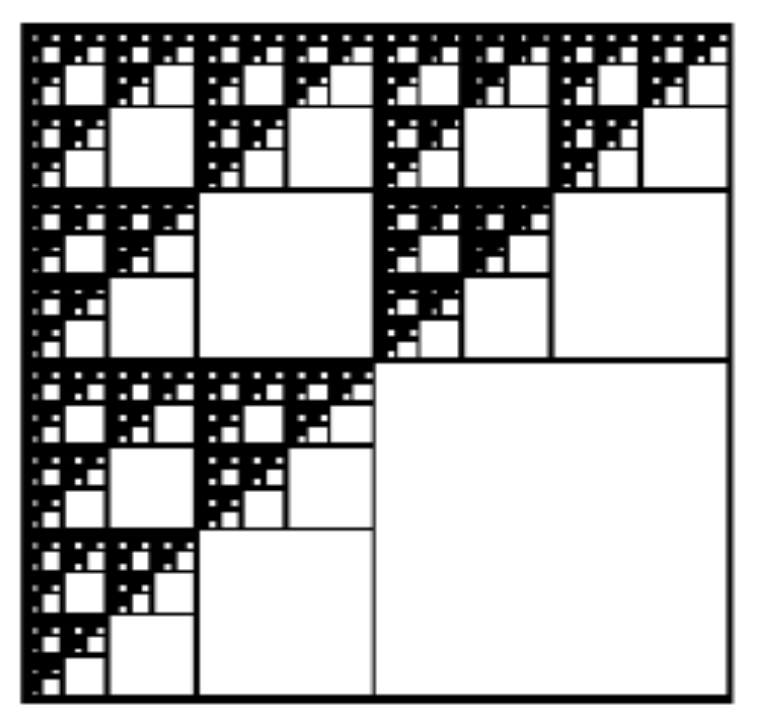
\includegraphics[width=0.3\textwidth]{myciel.png}} \quad
    \subfloat[]{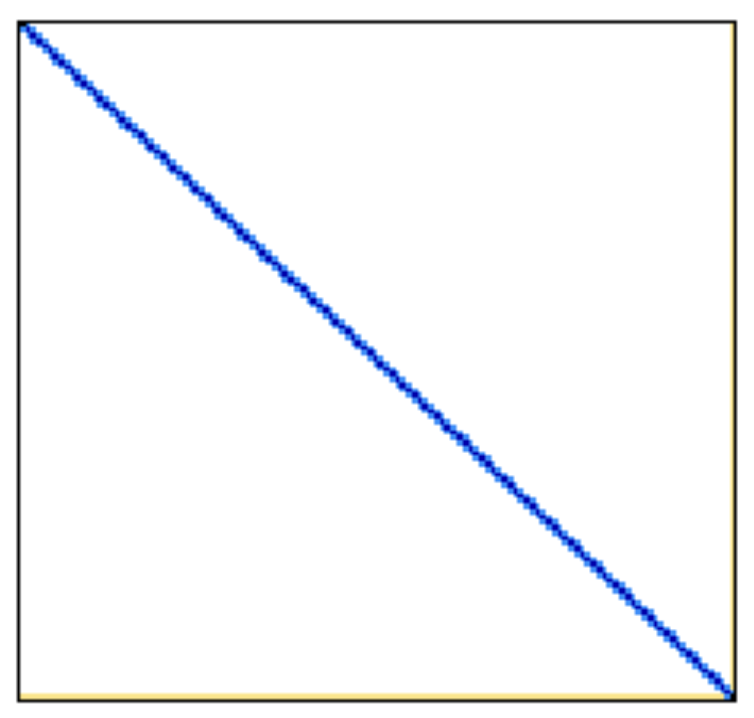
\includegraphics[width=0.3\textwidth]{hardesty.png}}\quad
    \subfloat[]{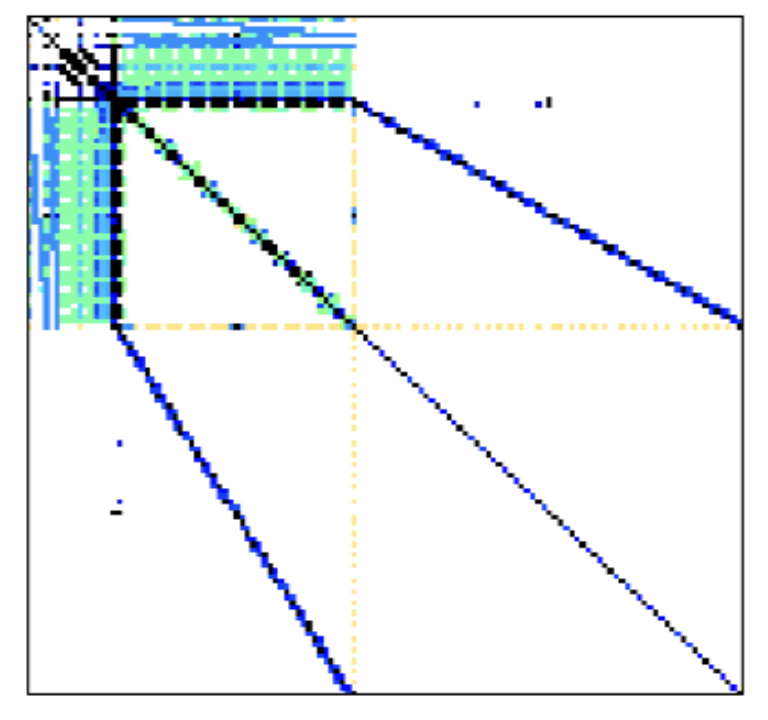
\includegraphics[width=0.3\textwidth]{memchip.png}}
    \caption{Matrices used for testing: (a) Mycielskian15, (b) Hardesty1, (c) Memchip}
\end{figure}
    \subsection{Load Balance comparison}
    If we compute the load imbalance as the difference between the maximum and minimum number of assigned non-zeros for each thread, we can compare the two load balancing strategies and see which gives us the best load balance.
    \medskip

    

    The following charts illustrate the load imbalance of these three matrices. 

    \begin{figure}[H]
        \begin{center}
            \includegraphics[width=0.95\textwidth]{mycimg.png}
        \end{center}
        \caption{Load imbalance of Mycielskain15}
    \end{figure}

    \begin{figure}[H]
        \begin{center}
            \includegraphics[width=0.95\textwidth]{memimb.png}
        \end{center}
        \caption{Load imbalance of memchip}
    \end{figure}

    \begin{figure}[H]
        \begin{center}
            \includegraphics[width=0.95\textwidth]{hardimb.png}
        \end{center}
        \caption{Load imbalance of Hardesty1}
    \end{figure}


\end{document}
